%% This is file `elsarticle-template-1-num.tex',
%% %% Copyright 2009 Elsevier Ltd
%%
%% This file is part of the 'Elsarticle Bundle'.
%% ---------------------------------------------
%%
%% It may be distributed under the conditions of the LaTeX Project Public
%% License, either version 1.2 of this license or (at your option) any
%% later version.  The latest version of this license is in
%%    http://www.latex-project.org/lppl.txt
%% and version 1.2 or later is part of all distributions of LaTeX
%% version 1999/12/01 or later.
%%
%% The list of all files belonging to the 'Elsarticle Bundle' is
%% given in the file `manifest.txt'.
%%
%% Template article for Elsevier's document class `elsarticle'
%% with numbered style bibliographic references
%%
%% $Id: elsarticle-template-1-num.tex 149 2009-10-08 05:01:15Z rishi $
%% $URL: http://lenova.river-valley.com/svn/elsbst/trunk/elsarticle-template-1-num.tex $
%%

%\documentclass[]{article} %\documentclass[final,3p,12pt]{elsarticle}
%\documentclass[final,12pt,times]{elsarticle}

%% Use the option review to obtain double line spacing
\documentclass[preprint,review,12pt]{elsarticle}

%% Use the options 1p,twocolumn; 3p; 3p,twocolumn; 5p; or 5p,twocolumn
%% for a journal layout:
%% \documentclass[final,1p,times]{elsarticle}
%% \documentclass[final,1p,times,twocolumn]{elsarticle}
%% \documentclass[final,3p,times]{elsarticle}
%% \documentclass[final,3p,times,twocolumn]{elsarticle}
%% \documentclass[final,5p,times]{elsarticle}
%% \documentclass[final,5p,times,twocolumn]{elsarticle}

\usepackage{amssymb}
\usepackage{wrapfig}
\usepackage{lipsum}
\usepackage{natbib}

\usepackage{tikz}
\usetikzlibrary{shapes, arrows}

\tikzstyle{notary} = [rectangle, draw, text centered, text width=4em, fill=blue!20, minimum height=2em]
\tikzstyle{user}   = [rectangle, draw, text centered, text width=4em, fill=green!20, minimum height=2em]
\tikzstyle{server} = [rectangle, draw, text centered, text width=4em, fill=red!20, minimum height=2em]
\tikzstyle{single}   = [draw, -latex']
\tikzstyle{double}   = [draw, latex-latex']

% http://tex.stackexchange.com/questions/35712/modify-footer-used-by-elsarticle-cls
\makeatletter
\def\ps@pprintTitle{
    \let\@oddhead\@empty
    \let\@evenhead\@empty
    \def\@oddfoot{\centerline{\thepage}}
    \let\@evenfoot\@oddfoot}
\makeatother

\journal{University of Guelph; CIS*4110}

\begin{document}

\begin{frontmatter}

\title{Improving Perspectives by adding functionally to update record of SSL certificates upon request}

\author[doug]{Douglas Anderson}
\author[eric]{Eric Boyd}
\author[james]{James Kelly}
\address[doug]{dander01@uoguelph.ca}
\address[eric]{boyde@uoguelph.ca}
\address[james]{kellyj@uoguelph.ca}


\begin{abstract}

Today's web is secured with SSL and TLS, which utilizes RSA to create secure
connections between servers and users. To ensure that the users are
communicating with the web server they intend and not someone masquerading as
the server, Certificate Authorities (CAs) are considered to be secure trusted
parties that can confirm the identity of the server. However, CAs
 can be compromised leaving users vulnerable. In an effort to fix the
weaknesses in the central authorities, The Perspectives Project uses a
constellation of Notary Servers spread out across the Internet to monitor the
SSL certificate signatures over time. Users install a web browser extension that
compares the signature of the certificate given to them from the server to the
certificates observed by the notaries. Our augmentation to the Perspectives
system allows web servers being monitored by a number of Notaries to send a
message to each of the Notaries when the server changes their SSL certificate.
This mitigates the lag between the certificate change and observation better
protecting users.

\end{abstract}

\begin{keyword}
% keywords here, in the form: keyword \sep keyword
Security \sep
SSL \sep
Central Authorities \sep
Perspectives
\end{keyword}

\end{frontmatter}

\section{Background}
\label{background}

In the modern world the Internet holds a very important role in commerce and
social aspects of life. Both of these pursuits require the ability for two or
more parties to communicate securely. To facilitate this secure communication,
the Internet has resorted to using the SSL (Secure Socket Layer) and it
successor TLS (Transport Security Layer) to protect the data being exchanged.
These protocols utilize public-private key pairs to facilitate RSA encryption.
While this protocol has been extremely successful it must rely on a CA to
confirm the identity of the owner of public keys. While it is possible to
create `self-signed' certificates browsers will warn users if a site uses one
of these certificate since it is impossible to verify who created the
certificate. 

Certificate Authorities are is a single point of failure in this authentication
system, and has in the past been compromised, allowing successful impersonation
of several popular, high profile websites.  In 2011 the central authority
Comodo Group, Inc. was hacked and the hacker made off with a SSL certificates
for various sites including Gmail, Yahoo Mail, Hotmail.  \citep{comodohack}
This would allow the hacker to preform man in the middle attacks on the sites
and read the emails of users of these services. The attack was easily executed
because of Comodo's extremely weak password that was easily broken with a word
list. This illustrates the vulnerability in the SSL protocol that central
authorities create.

This is vulnerability is what the Perspectives project set out to fix. Their
solution to removing central authorities is to create trusted services known as
notaries. These notaries work in tandem with a browser extension that allows
users of the extension to select which of the notaries they would like to
trust. The system works by checking the SSL certificate signature that they are
given from the server against the SSL certificates signatures that the users
trusted notaries have in their databases. If there is a discrepancy between the
certificate signature that the server has returned and the signatures that the
notaries have on record, the SSL connection is aborted.

\begin{figure}[h]
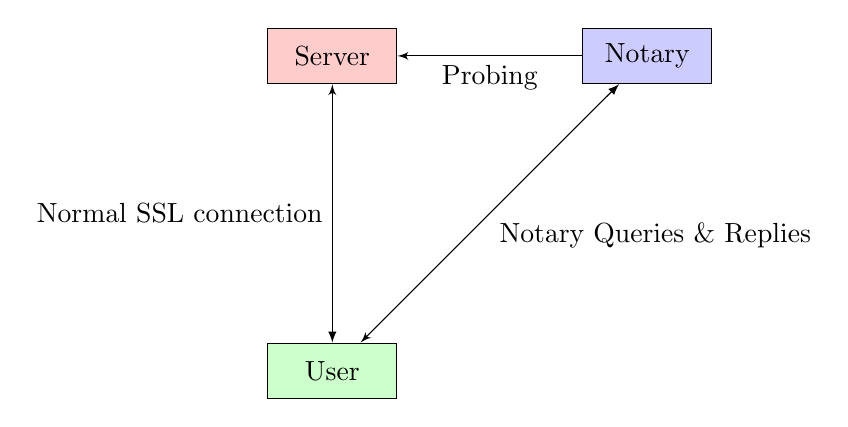
\begin{tikzpicture}[node distance = 4cm, auto]
    \node[server](server){Server};
    \node[notary, right of=server](note){Notary};
    \node[user, below of=server](user){User};
    \path[double](note) -- node {Notary Queries \& Replies}(user);
    \path[double](user) -- node {Normal SSL connection}(server);
    \path[single](note) -- node {Probing}(server);
\end{tikzpicture}
\caption{Normal Performance of the perspectives system.}
\end{figure}

\section{Implementation}
\label{implementation}

We attempted to build upon the Perspective Project by allowing
servers to send messages to notaries requesting that the notary make note of
the change of SSL certificate. This fixes the problem in the perspectives
project that can occur when a server changes it's SSL certificate and a user
queries the notary for that server's SSL certificate. Because the notary has
not yet updated it's record of the SSL certificate and reports to the user that
there is a mismatch which may lead the user to abort their attempt to create an
SSL connection.

For a server notify Perspectives notary it must first know that the notary
exists. To facilitate this we added a user agent string to the notaries
scanning facilities. This allows notary aware web servers to add any users with
the Notary user agent string to the list of known notaries. In our
implementation the notaries user agent string was:

\begin{verbatim}
    Perspectives-Notary/4.4
\end{verbatim}

\begin{figure}[h]
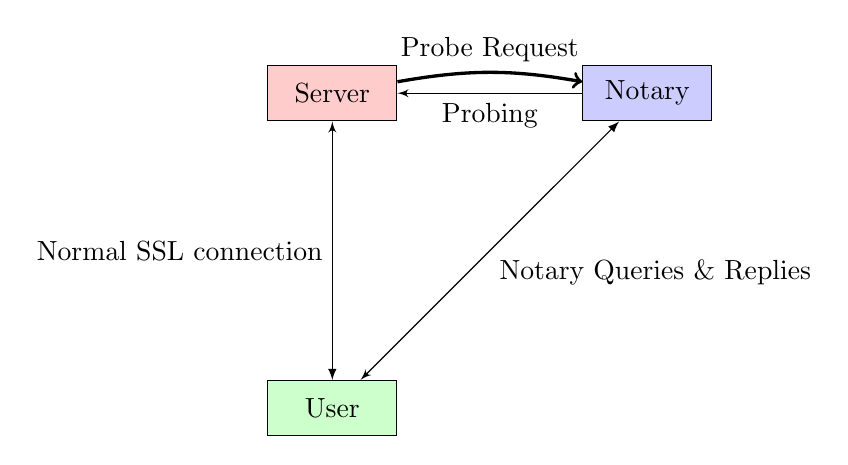
\begin{tikzpicture}[node distance = 4cm, auto]
    \node[server](server){Server};
    \node[notary, right of=server](note){Notary};
    \node[user, below of=server](user){User};
    \path[double](note) -- node {Notary Queries \& Replies}(user);
    \path[double](user) -- node {Normal SSL connection}(server);
    \path[single](note) -- node {Probing}(server);
    \path[->](server) edge[very thick, bend left=10] node{Probe Request}(note);
\end{tikzpicture}
\caption{Our modified perspective notary allows for the server to request that
    it's SSL certificate be probed and updated in the Notaries Database.}
\end{figure}

When a server changes it's SSL certificate, it sends an HTTP request to all of
the notaries it is aware of. Due to the distributed nature of the notaries, the
change is permitted to propagate within the notary network. In our
implementation we used extended the query string of the HTTP GET requests that
the perspective server. The request is in the following form:


\begin{verbatim}
    http://<Notary URL>/?host=<Server URL>&update=certificate
\end{verbatim}

Notary web-crawlers make themselves known to webservers, by setting a custom
HTTP user-agent string, similar to how Google and other search engine's
web-crawlers function. If webservers take note of the notaries checking their
certificates, by checking for this user-agent string, they know how recent their
SSL certificate entry is within the notary network system.

\section{Results}
\label{results}

\section{Conclusion}
\label{conclusion}

\section{Further Work}
\label{further work}

\subsection{Add preventive measures against DOS}

Since it is relatively computationally expensive for the notary to probe a
server for a SSL certificate signature it is possible to use these requests to
make a particular notary unresponsive to user queries. This could allow an
attacker to perform a man in the middle attack by rendering all of a users
notaries unresponsive before beginning their attack. While it may be possible
to prevent this attack on the part of the user by not continuing with the SSL
connection when none of their trusted notaries respond, This would still be
undesirable since it would prevent the user from making any secure connections.

\begin{enumerate}
    \item {Only probe a server when the probe request comes from the server itself}

        By only probing a server when the request comes from the server itself
        the possibility of external abuse is extremely limited. This method may
        be hard to implement in practise because it is possible for the
        attackers to spoof the origin of probe request to be the IP of the
        server.

    \item {Rate limit probe requests}

        By only allowing a certain number of probe requests in a period of time
        the notary can ensure that it does not compromise it's ability to
        respond to user request. This a common DOS prevention technique because
        of how effective it is, however it is possible that this method would
        become swamped at certain times since many websites change their SSL
        certificate at times of low traffic (e.g. 3AM).

\end{enumerate}

\section{References}
\label{references}
\nocite{*}
\bibliographystyle{plainnat}
\bibliography{report}

\end{document}

